\section{Organisatorisches}

Prof. Rennekamp (N228)\\
rennekamp@mw.htw-dresden.de

Prüfung WS + Prüfung SS = Modulnote Technische Physik

4 Praktika

Zur Prüfung ist alles an Unterlagen etc. erlaubt.

Literaturempfehlung: Physik Der Grundkurs ISBN: 978-3-8085-5621-4

\subsection{Gliederung des Semesters}
\begin{enumerate}
	\item Mechanik
	\item Schwingungen und Wellen
	\item Optik
	\item (Wärmelehre)
	\item (Atom und Festkörperphysik)
\end{enumerate}

\section{Mechanik}

Kinematik der Punktmasse

Bewegung einer Punktmasse im Raum

Einfachster Fall:

\begin{minipage}{.5\textwidth}
		$$x = x(t)$$
		$$y = y_0 = const.$$
		$$z = z_0 = const.$$
\end{minipage} \hfill
\begin{minipage}{.45\textwidth}
	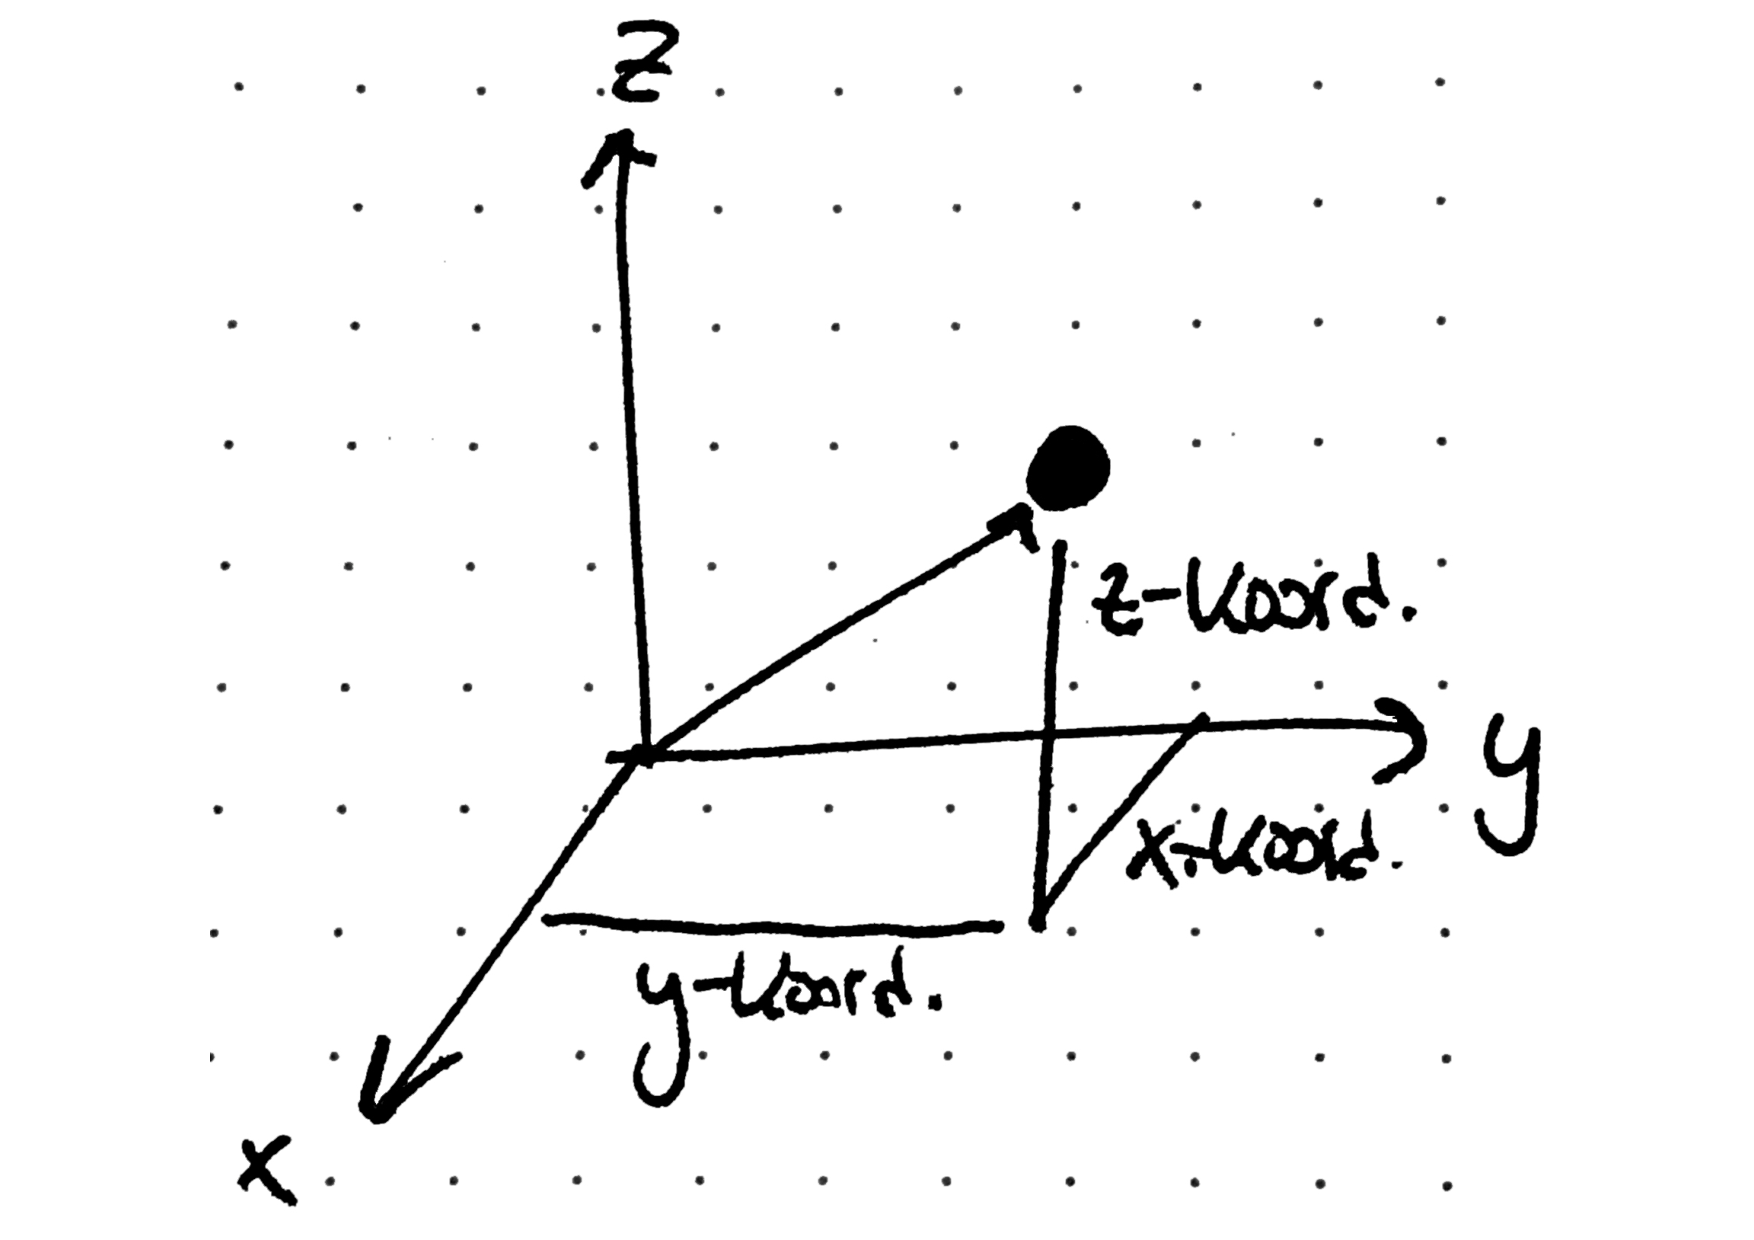
\includegraphics[width=\textwidth]{img/1_1}
\end{minipage}

Bezugssystem kartesisches Koordinatensystem

\Ra eindimensionale Bewegung

\underbar{Rechte-Hand-Regel:}
\begin{itemize}
	\item Daumen: x ($x_1$)
	\item Zeigefinger: y ($x_2$)
	\item Mittelfinger: z ($x_3$)
\end{itemize}

\newpage

\underbar{Versuch:} Körper im Zustand der Ruhe

Ohne äußere Einwirkung keine Bewegung $s(t) = s_0$

\begin{center}
	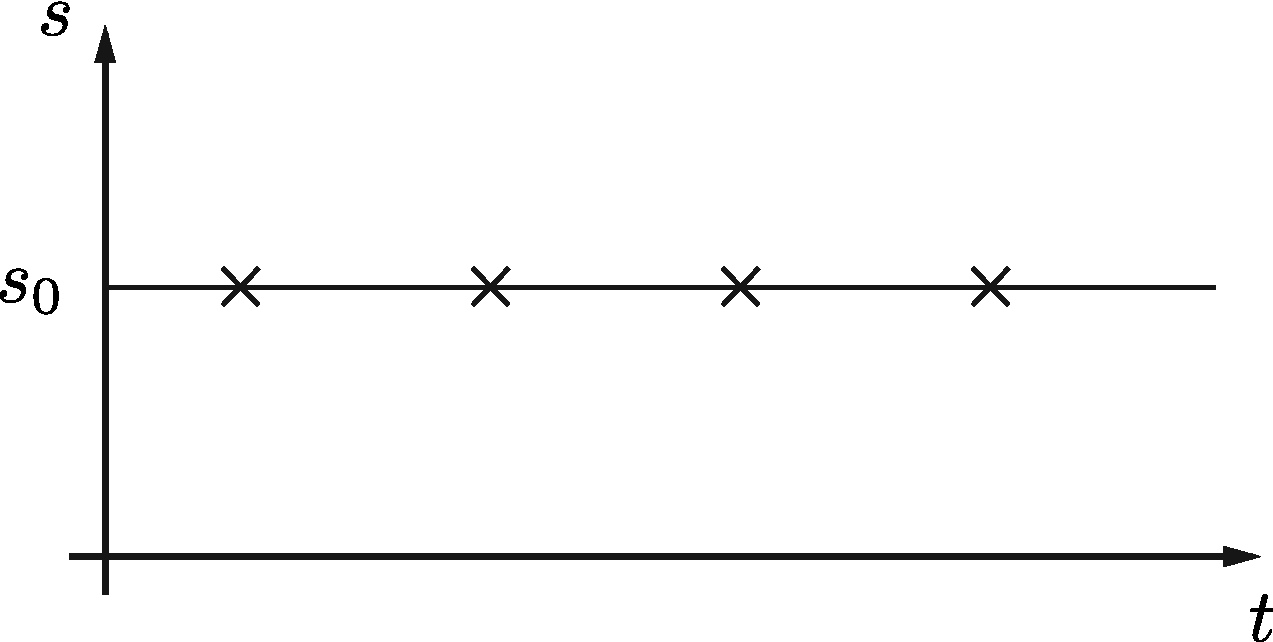
\includegraphics[width=.6\textwidth]{img/1_2}
\end{center}

\underbar{Versuch:} Geradlinig gleichförmige Bewegung

\begin{minipage}{.5\textwidth}
	\begin{tabular}{| c | c | c |}
		\hline
		Weg & Messung 1 & Messung 2\\
		$s(t)$ & $t$ & $t$ \\
		\hline
		0,2 & 0,41 & 0,79 \\
		0,4 & 0,84 & 1,53 \\
		0,6 & 1,26 & 2,28 \\
		0,8 & 1,65 & 3,02 \\
		\hline
	\end{tabular}
\end{minipage} \hfill
\begin{minipage}{.5\textwidth}
	\hspace{0.45cm} % Because pushing stuff around with hspaces to line it up isn't stupid at all
	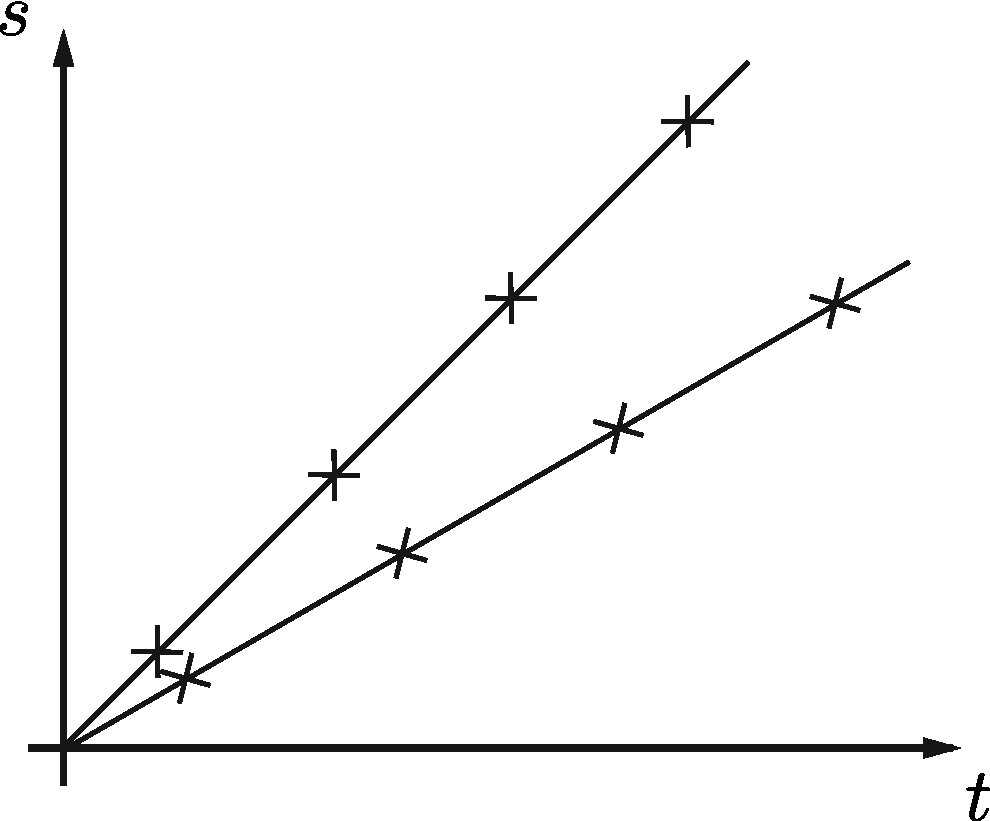
\includegraphics[width=.7\textwidth]{img/1_3}
\end{minipage}

$s(t) = s_0 + v \cdot t$ mit der Geschwindigkeit $v = \frac{\Delta s}{\Delta t} = const.$ wurde für zwei Geschwindigkeiten ($v_1 > v_2$) realisiert.

\underbar{Versuch:} Geradlinig gleichmäßig beschleunigte Bewegung

\begin{minipage}{.5\textwidth}
	\begin{tabular}{| c | c | c |}
		\hline
		Weg & Messung 1 & Messung 2\\
		$s(t)$ & $t$ & $t$ \\
		\hline
		0,2 & 1,26 & 2,50 \\
		0,4 & 1,86 & \\
		0,6 & 2,33 & \\
		0,8 & 2,74 & 5,35 \\
		\hline
	\end{tabular}
\end{minipage} \hfill
\begin{minipage}{.5\textwidth}
	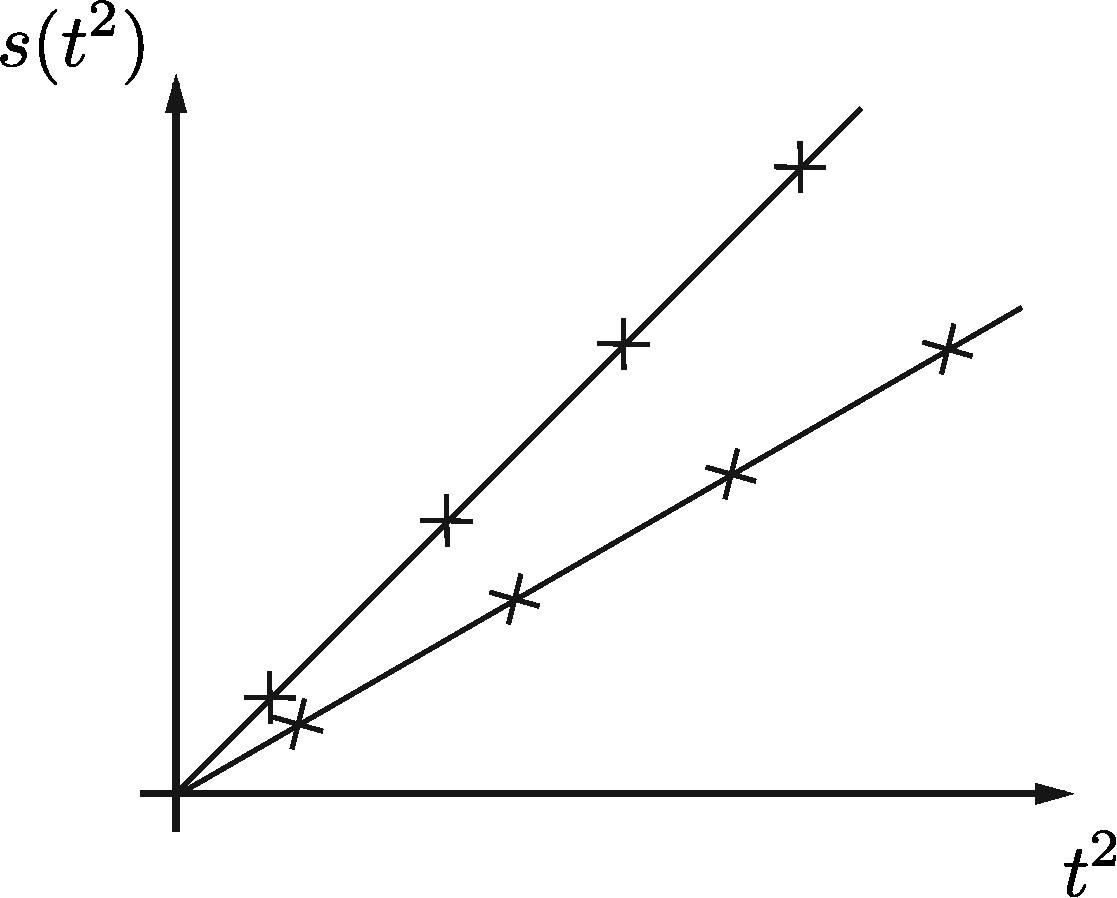
\includegraphics[width=.8\textwidth]{img/1_4}
\end{minipage}

Ergebnis: $s(t) = s_0 + 0,5at^2$ mit der Geschwindigkeit $v = \lim_{\Delta t \to 0} \frac{\Delta s}{\Delta t} = at$ und der Beschleunigung $a = \frac{\Delta v}{\Delta t} = const.$ wurde für zwei Beschleunigungen ($a_3 < a_4$) realisiert.
